


本章では,Webシステムにおける測定値閲覧機能について説明する.
本研究室で稼働しているサーバにはWebシステムが設置されており,URLを通じてアクセスすることができる.
測定値閲覧機能は,測定機器の種類や閲覧するデータの内容によって異なるため,複数のシステムが作成されている.
基本的な構成としては,測定機器で測定された値の一覧と測定時間をカラムに持つ表形式と,測定値を可視化したチャート形式の2種類の表示方法を採用している.
チャートの描画には,JavaScriptのフレームワークであるChart.jsを使用している.
以下では,各Webシステムの詳細について述べる.

\section{Arduino用測定値閲覧機能}
Arduino用測定値閲覧機能を,図\ref{fig:ArduinoAirflowChart},図\ref{fig:nowAirflowData}に示す.
データベースに保存された測定値はPHPで取得され,そのデータがJavaScriptにJSON形式で渡されており,
表形式とチャート形式の両方で測定値を表示することができる.
チャートには風速の最大値が表示されている.
更新頻度は約10秒で,最新のデータが取得される仕組みとなっている.


\begin{figure}[h]
\centering
\begin{minipage}{0.49\linewidth}
    \centering
    \includegraphics[width=\linewidth]{./figures/ArduinoAirflowChart}
    \caption{Arduino Airflow Chart}
    \label{fig:ArduinoAirflowChart}
\end{minipage}
\begin{minipage}{0.49\linewidth}
    \centering
    \includegraphics[width=\linewidth]{./figures/nowAirflowData}
    \caption{Now Airflow Data}
    \label{fig:nowAirflowData}
\end{minipage}
\end{figure}

\section{ESP32C6用測定値閲覧機能}
ESP32C6用測定値閲覧機能を,図\ref{fig:webAirGraph},図\ref{fig:webAirTb}に示す.
このWebシステムでは全ての測定値にチャートを対応させた.
チャートの左にある項目から各測定値に表示を切り替えることができる.
更新頻度は約20秒で,表とチャートには100件分の最新データが取得される仕組みとなっている.

\begin{figure}[h]
\centering
\begin{minipage}{0.49\linewidth}
    \centering
    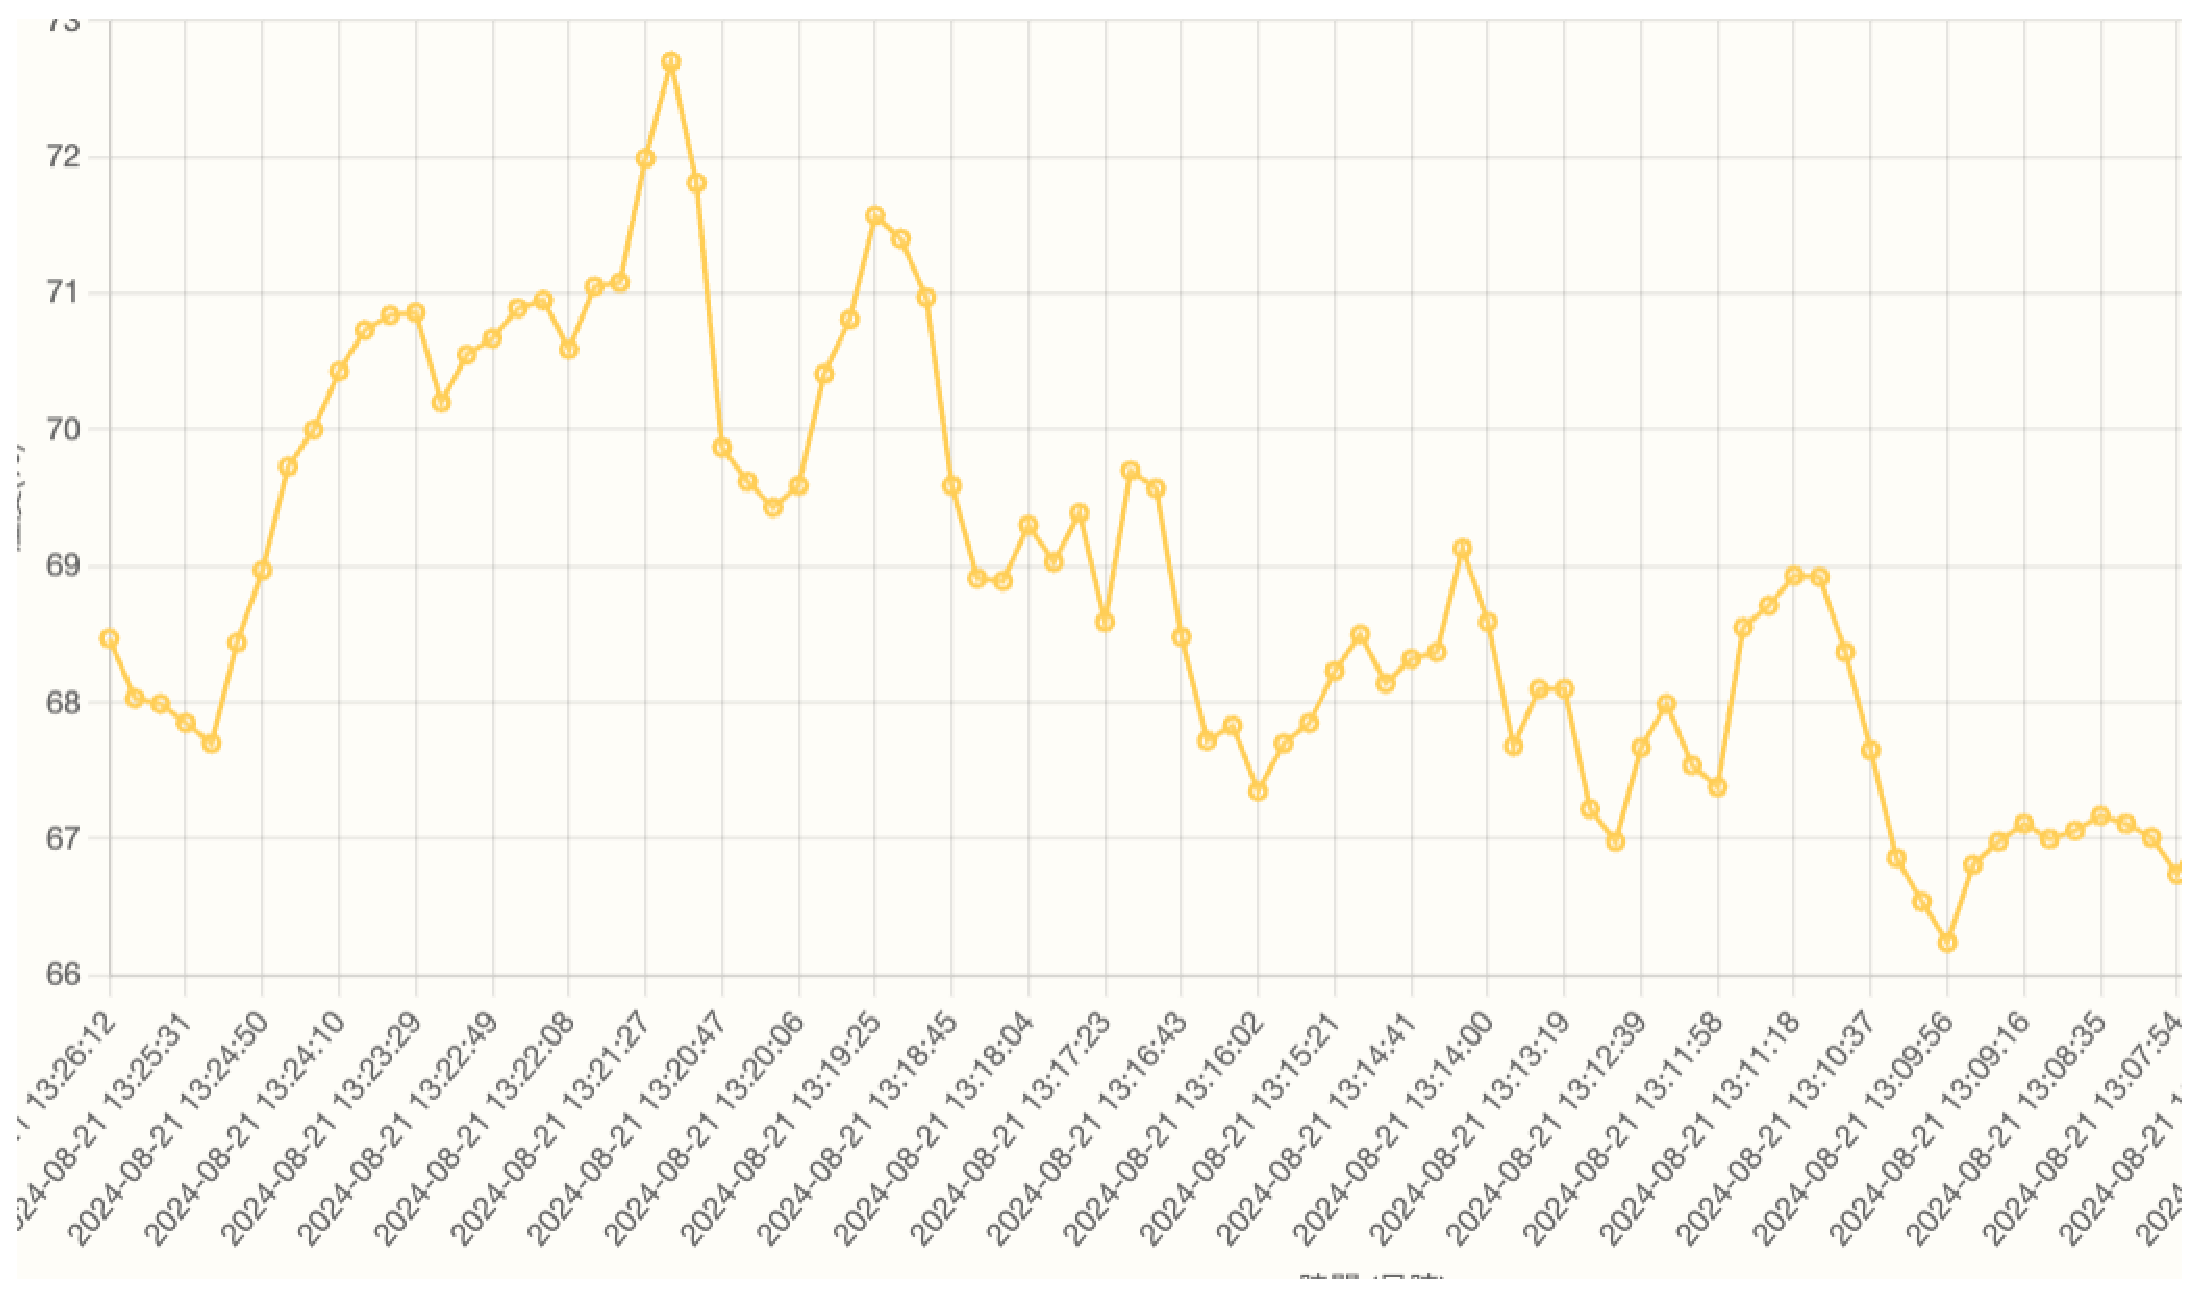
\includegraphics[width=\linewidth]{./figures/webAirTb.eps}
    \caption{測定を表示するグラフ}
    \label{fig:webAirGraph}
\end{minipage}
\begin{minipage}{0.49\linewidth}
    \centering
    \includegraphics[width=\linewidth]{./figures/airTabTable.eps}
    \caption{過去100件の実測値を表示する表}
    \label{fig:webAirTb}
\end{minipage}
\end{figure}




\section{同時に全項目を表示}
同時に全項目を表示する機能を図\ref{fig:airflowCharts}に示す.
このWebシステムは上の項のWebシステムの仕様を変更したバージョンで,同時に一つの項目しか見れなかったものを全ての測定値の項目を一度に見れるようにしたものである.
仮に測定値の項目が増減しても自動で項目も増減し対応する.
更新頻度などは同じ仕様で設計している.

\begin{figure}
\centering
\includegraphics[width=1\linewidth]{./figures/airflowCharts}
\caption{airflowCharts}
\label{fig:airflowCharts}
\end{figure}



\section{デバイスごとの測定値を表示}
デバイスごとの測定値を表示する機能を図\ref{fig:WebSystemESPDeviceIds}に示す.
このWebシステムはこれまで全てのデバイスの測定値を一見の測定値として扱っていたものをデバイスごとに表示する目的で作成した.
ドロップダウンリストでデバイスを選択できること以外仕様は同じ.



\begin{figure}
\centering
\includegraphics[width=1\linewidth]{./figures/WebSystemESPDeviceIds}
\caption{測定機器ごとの測定値を表示するグラフ}
\label{fig:WebSystemESPDeviceIds}
\end{figure}

\section{デバイスをグループ分けして表示}
デバイスをグループ分けして表示する機能を図\ref{fig:ESPGroupGraph}に示す.
このWebシステムはデバイスをグループ分けしてグループごとにグラフを出せるようにしたもの.
専用のページからグループを作成し,デバイスをグループ分けをすることでWebシステムに追加される.
このWebシステムは過去1時間のデータを取得し,20秒ごとに情報を更新する.

\begin{figure}
\centering
\includegraphics[width=1\linewidth]{./figures/ESPGroupGraph}
\caption{グループごとの測定値を表示するグラフ}
\label{fig:ESPGroupGraph}
\end{figure}




\section{冷暖房能力の閲覧機能}

本項では,冷暖房能力の閲覧機能について図\ref{fig:CoolingCapability}に示す.
本機能は空調機器の性能を評価し,表示するために開発を行った.
空調機の冷暖房能力を計算し,その結果をリアルタイムで表示することができる.
このシステムは吹出口の風速,温度,湿度,および吸込口の温度を元に顕熱および潜熱を計算し,
その合計を全熱とし,空調設備の冷暖房能力を表示する.
空調能力に関しては,空調のモデルによって異なるため,モデルに合わせた計算式を使用している.
今回は,本研究室に設置されている\textbf{PLFY-P112EMC6}のモデルに合わせた計算式を使用している.


\subsection*{計算式}

\subsubsection*{顕熱}
顕熱は以下の式で計算する.
\[
Q = V \times \rho \times c \times \Delta T
\]

各項の定義を以下に示す.
\begin{align*}
\rho &= 1.2\,\mathrm{kg/m^3} & \text{(空気密度)} \\
c &= 1.006\,\mathrm{kJ/(kg \cdot K)} & \text{(空気の定圧比熱)} \\
V &= \text{風量(変換後の}\,\mathrm{m^3/s}\text{)} \\
\Delta T &= \text{吸込口と吹出口の温度差}
\end{align*}

\subsubsection*{潜熱}
潜熱も以下の式で計算する.
\[
Q' = V \times \rho \times \Delta h
\]

\subsubsection*{全熱}
 \[
Q_{\text{total}} = Q + Q' = \left( V \times \rho \times c_a \times \Delta T \right) + \left( V \times \rho \times \Delta h \right)
\]


ここで,\(\Delta h\)は比エンタルピーの差を表し,以下の関係で求める.
\[
\Delta h = h_2 - h_1
\]

\begin{align*}
h_1 &= c_a \cdot t_1 + x_1 \cdot (\gamma_o + c_w \cdot t_1) & \text{(吸込口の比エンタルピー)} \\
h_2 &= c_a \cdot t_2 + x_2 \cdot (\gamma_o + c_w \cdot t_2) & \text{(吹出口の比エンタルピー)}
\end{align*}

各項の定義は以下の通りである.
\begin{align*}
t_1 &= \text{吸込口温度(}\mathrm{^\circ C}\text{)}, &
t_2 &= \text{吹出口温度(}\mathrm{^\circ C}\text{)}, \\
x_1 &= \text{吸込口の絶対湿度(}\mathrm{kg/kg(DA)}\text{)}, &
x_2 &= \text{吹出口の絶対湿度(}\mathrm{kg/kg(DA)}\text{)}.
\end{align*}

以下の定数を用いる.
\begin{align*}
c_a &= 1.006\,\mathrm{kJ/(kg(DA) \cdot K)} & \text{(乾き空気の定圧比熱)}, \\
c_w &= 1.805\,\mathrm{kJ/(kg(DA) \cdot K)} & \text{(水蒸気の定圧比熱)}, \\
\gamma_o &= 2501\,\mathrm{kJ/kg} & \text{(水の蒸発潜熱)}.
\end{align*}

\begin{figure}[h]
\centering
\includegraphics[width=1\linewidth]{./figures/CoolingCapability}
\caption{冷暖房能力の閲覧機能}
\label{fig:CoolingCapability}
\end{figure}


